\subsection{Projected gamma family\label{subsec:projgamma}}
  A natural  distribution to consider in ${\mathbb R}^p_+$ is given by a product of independent
  univariate Gamma distributions. Let
    $\bm{ X} \sim \prod_{\ell = 1}^d\text{Ga}\left(X_{\ell}\mid\alpha_{\ell},\beta_{\ell}\right)$, 
    $\alpha_\ell$ and $\beta_\ell$ are the shape and scale parameters, respectively. Using Equations (\ref{eqn:pnormt}) -- (\ref{eqn:pnormjac}) we have the joint density
  \begin{equation}
  \label{joint}
    f(r,\bm{ y}) = \prod_{\ell = 1}^{d}
      \left[\frac{\beta_{\ell}^{\alpha_{\ell}}}{\Gamma(\alpha_{\ell})}(ry_{\ell})^{\alpha_{\ell} - 1}
          \exp\lbrace-\beta_{\ell}ry_{\ell}\rbrace\right]
      \times r^{d-1}\left[y_d +
            {\textstyle \sum}_{\ell = 1}^{d-1}y_{\ell}^p\left(y_d^p\right)^{\frac{1}{p} - 1}\right].
  \end{equation}
  Integrating out $r$ yields the resulting \emph{Projected Gamma} density
  \begin{equation}
    \label{eqn:projgamma}
    \text{PG}(\bm{ y}\mid\bm{ \alpha},\bm{ \beta}) =
          \prod_{\ell = 1}^d\left[\frac{\beta_{\ell}^{\alpha_{\ell}}}{\Gamma(\alpha_{\ell})}
                y_{\ell}^{\alpha_{\ell} - 1}\right]
      \times \left[y_d +
          {\textstyle \sum}_{\ell = 1}^{d-1}y_{\ell}^p\left(y_d^p\right)^{\frac{1}{p} - 1}\right]
      \times \frac{\Gamma({\textstyle\sum}_{\ell = 1}^d\alpha_{\ell})}{\left({\textstyle\sum}_{\ell = 1}^d
                    \beta_{\ell}y_{\ell}\right)^{{\scriptstyle\sum_{\ell = 1}^d \alpha_{\ell}}}} ,
  \end{equation}
  defined for $\bm{y}\in {\mathbb S}_p^{d-1}$, and for any $p>0$. To avoid identifiability problems when estimating the shape and scale parameters, we set $\beta_1 = 1$.
  \cite{nunez2019} obtain the density in Equation (\ref{eqn:projgamma})
  for $p=2$ as a multivariate distribution for directional data, using spherical coordinates.
  For $\bm{ y}\in {\mathbb S}_1^{d-1}$, and $\beta_{\ell} = \beta$ for all $\ell$, the density in Equation (\ref{eqn:projgamma}) corresponds to that of a Dirichlet distribution.
  
  The projected gamma family is simple to specify and has very tractable computational properties. Thus, we use it as a building block for the angular measure $\Phi$ models. To build a flexible family of distributions in ${\mathbb S}_p^{d-1}$ we consider mixtures of projected gamma densities defined as
  \begin{equation} \label{eqn:PGmix}     
     f(\bm{y}) = \int_\Theta \mathcal{PG}(\bm{y}|\bm{\theta}) dG(\bm{\theta}), 
  \end{equation} 
  where $\bm{\theta} = (\bm{\alpha}, \bm{\beta})$. Following a Bayesian non-parametric approach \citep{Ferguson74,Antoniak1974} we assume that $G$ is drawn from a random measure. In particular, assuming a Dirichlet process prior, we have a hierarchical formulation of the mixture model that, for a vector of observations $\bm{y}_i$, is given by
  \begin{equation}\label{eqn:dppg}    \bm{y}_i \sim \text{PG}(\bm{y}_i|\bm{\theta}_i) , \;\;\; \bm{\theta}_i \sim G, \;\;\; G \sim \mathcal{DP}(\eta, G_0),
  \end{equation}
  where $\mathcal{DP}$ denotes a Dirichlet process, $\eta$ is the precision parameter, and $G_0$ is the centering distribution. 
  
  Our strategy consists of describing the angular distribution $\Phi$ using a sample based approach with the following steps: (i) Apply the transformation in Equation (\ref{eqn:standardization}) to the original data; (ii) Obtain the subsample of the standardized observations that satisfy $R>1$; (iii) Take a finite $p$ and project the observations onto ${\mathbb S}_p^{d-1}$; (iv) Fit the model in Equation (\ref{eqn:PGmix}) to the resulting data and obtain samples from the fitted model; (v) Project the resulting samples onto ${\mathbb S}_\infty^{d-1}$.
  For step (iv) we use a Bayesian approach that is implemented using a purposely developed Markov chain Monte Carlo that is described in the next section.

\begin{figure}[ht]
    \centering
  \begin{subfigure}[b]{0.47\textwidth}
    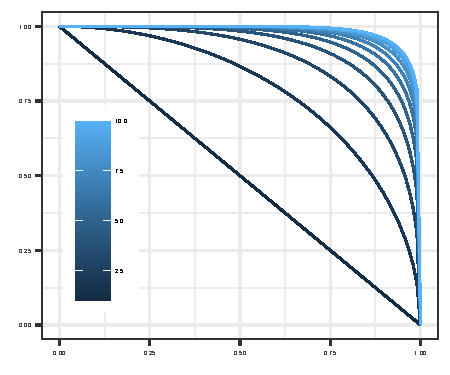
\includegraphics[width=\textwidth]{./images/p_sphere}
    \caption{${\mathbb S}_p^1$ for $p = 1,\ldots, 10$\label{fig:psphere}}
  \end{subfigure}
  %
  \begin{subfigure}[b]{0.47\textwidth}
    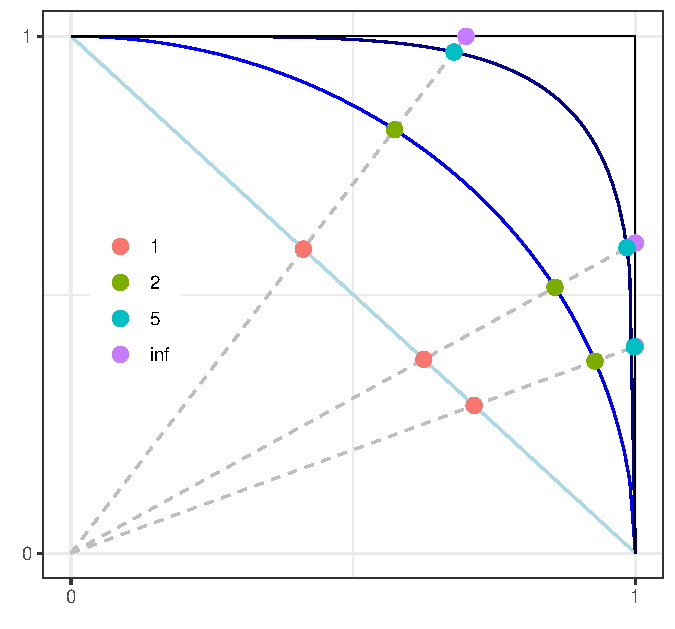
\includegraphics[width=\textwidth]{./images/p_project}
    \caption{Projection of data on ${\mathbb S}_{\infty}^1$ onto ${\mathbb S}_p^1$\label{fig:pproject}}
  \end{subfigure}
\end{figure}

\subsubsection{Inference for the projected Gamma mixture model}
The Dirichlet process mixture model groups observations into stochastically assigned \emph{clusters}.  Building out the methods of inference for Equation~\ref{eqn:dppg}, let $n_j^{-i}$ be the number of observations in cluster $j$ not including observation $i$.  Let $J^{-i}$ be the number of extant 
% {\bf (remaining?)} observations
clusters, not including any singleton that observation $i$ is in. Under this model, the probability of cluster membership for a given observation is proportional to
\begin{equation*}
    \text{Pr}\left[\delta_i = j\mid\ldots\right] \propto \begin{cases}
        n_j^{-i}\mathcal{PG}\left(\bm{y}_i\mid\bm{\alpha}_j,\bm{\beta}_j\right)\hspace{0.5cm} &\text{~for~}j \in \lbrace 1,\ldots,J^{-i}\rbrace\\
        \eta\int\mathcal{PG}\left(\bm{y}_i\mid\bm{\alpha}_j,\bm{\beta}_j\right)dG_0(\bm{\alpha}_j,\bm{\beta}_j)\hspace{0.5cm} &\text{~for~}j = J^{-i} + 1.
        \end{cases}
\end{equation*}
If $G_0$ is not a conjugate prior for the kernel, the integral in the above formula may not be
available in closed form. Using Algorithm 8 from \cite{neal2000}, by Monte Carlo integration, drawing  $m$ candidate
clusters, $\bm{\alpha}_j,\bm{\beta}_j$ for $j = J^{-i} + 1,\ldots, J^{-i} + m$ from $G_0$. 
Then, we sample the cluster indicator $\delta_i$ from extant or candidate clusters, where
the probability of cluster membership is proportional to
\begin{equation}
    \text{Pr}\left[\delta_i = j\mid\ldots\right] \propto \begin{cases}
        n_j^{-i}\mathcal{PG}\left(\bm{y}_i\mid\bm{\alpha}_j,\bm{\beta}_j\right)\hspace{0.5cm} &\text{~for~}j \in \lbrace 1,\ldots,J^{-i}\rbrace\\
        \frac{\eta}{m}\mathcal{PG}\left(\bm{y}_i\mid\bm{\alpha}_j,\bm{\beta}_j\right)\hspace{0.5cm} &\text{~for~}j \in \lbrace J^{-i} + 1,\ldots, J^{-i} + m\rbrace.
        \end{cases}
\end{equation}
If a candidate cluster is selected,
%{\bf you first have to say that you sample from this distribution. What is the ``candidate cluster''?}
then $\delta_i = J = J^{- i} + 1$, and the associated cluster parameters are saved.

A key feature of the the projected Gamma distribution is its computational properties. We augment  $\mathcal{PG}(\bm{y}_i\mid\bm{\alpha}_i,\bm{\beta}_i) $ by introducing a latent radial component $r_i$, for each observation. Using Equation \eqref{joint} we observe that the 
full conditional of $r_i$ is easy to sample from, as it is given as
\begin{equation}
    r_i\mid\bm{\alpha}_i,\bm{\beta}_i \sim \mathcal{G}\left(\sum_{\ell = 1}^d\alpha_{i\ell}, \sum_{\ell = 1}^d\beta_{\ell} y_{i\ell}\right).
\end{equation}
Moreover,  the full conditional for $\bm{\alpha}_j,\bm{\beta}_j$ is then proportional to
\begin{equation}
    f(\bm{\alpha}_j,\bm{\beta}_j\mid \bm{Y},\bm{r},\bm{\delta},\ldots) \propto \prod_{i:\gamma_i = j}\prod_{\ell = 1}^d\mathcal{G}\left(r_iy_{i\ell}\mid\alpha_{j\ell},\beta_{j\ell}\right) \times dG_0(\bm{\alpha}_j,\bm{\beta}_j).
\end{equation}
We first consider a centering distribution given by a product of independent Gammas:
\begin{equation*}
    G_0(\bm{\alpha}_j,\bm{\beta}_j\mid \bm{\xi},\bm{\tau},\bm{\zeta},\bm{\sigma}) = \prod_{\ell = 1}^d\mathcal{G}(\alpha_{j\ell}\mid \xi_{\ell},\tau_{\ell})\times\prod_{\ell = 2}^d\mathcal{G}(\beta_{j\ell}\mid\zeta_{\ell},\sigma_{\ell}).
\end{equation*}
This model is completed with independent Gamma priors on $\xi_{\ell}$, $\tau_{\ell}$, $\zeta_{\ell}$, $\sigma_{\ell}$.  We also assume a Gamma prior on $\eta$, that is updated via the procedure outlined in \cite{escobar1995}.  We refer to this model as the \emph{projected Gamma--Gamma} (PG--G) model.  An advantage of the PG--G model is that, thanks to conjugacy, the rate parameters can easily be integrated out for inference on $\bm{\alpha}_j$.  Then, the full conditional for $\alpha_{j\ell}$ takes the form
\begin{equation*}
    \pi(\alpha_{j\ell}\mid \bm{r},\bm{Y},\bm{\gamma},\xi_\ell,\tau_\ell,\zeta_\ell,\sigma_\ell) \propto \frac{\left(\prod_{i:\gamma_i = j}r_iy_{i\ell}\right)^{\alpha_{j\ell} - 1}\alpha_{j\ell}^{\xi_\ell - 1}e^{-\tau_\ell \alpha_{j\ell}}\times\Gamma\left(n_j\alpha_{j\ell} + \zeta_{\ell}\right)}{\Gamma^{n_j}(\alpha_{j\ell})\left(\sum_{i:\gamma_i = j}r_iy_{i\ell} + \sigma_{\ell}\right)^{n_j\alpha_{j\ell} + \zeta_{\ell}}}
\end{equation*}
for $\ell = 2,\ldots,d$.  For $\ell = 1$, as $\beta_{1} := 1$, the full conditional takes the form
\begin{equation}
    \label{eqn:alpha1update}
    \pi(\alpha_{j1}\mid\bm{r},\bm{Y},\bm{\gamma},\xi_1,\tau_1) \propto \frac{\left(\prod_{i:\gamma_i = j}r_iy_{i1}\right)^{\alpha_{j1} - 1}\alpha_{j1}^{\zeta_1 - 1}e^{-\tau_1\alpha_{j1}}}{\Gamma^{n_j}(\alpha_{j1})}.
\end{equation}
Sample of $\alpha_{j\ell}$ can thus be obtained using a Metropolis step. In our analysis, we first transform $\alpha_{j\ell}$ to the log scale, and use a normal proposal density.
The full conditional for $\beta$ is 
\begin{equation}
    \beta_{j\ell}\mid\bm{r},\bm{Y},\alpha,\zeta_{\ell},\sigma_{\ell} \sim \mathcal{G}\left(\beta_{j\ell}\mid n_j\alpha_{j\ell} + \zeta_\ell, \sum_{i:\gamma_i = j}r_iy_{i\ell} + \sigma_{\ell}\right),
\end{equation}
for $\ell = 2,\ldots, d$.  Updating $\beta_{j\ell}$ is done via a Gibbs step.  The hyper-parameters $\xi_{\ell},\tau_{\ell},\zeta_{\ell},\sigma_{\ell}$ follow similar Gamma-Gamma update relationships.  We also explore a restricted form of this model, where $\beta_{\ell} = 1$ for all $\ell$.  Under this model, we use the full conditional in Equation~\ref{eqn:alpha1update} for all $\ell$, and omit inference on $\bm{\zeta},\bm{\sigma}$.  We refer to this model as the \emph{projected restricted Gamma--Gamma} (PRG--G) model.

The second form of centering distribution we explore is a multivariate log-normal distribution on the shape parameters $\bm{\alpha}_j$, with independent Gamma $\beta_{j\ell}$ rate parameters.  
\begin{equation}
    G_0\left(\bm{\alpha}_j,\bm{\beta}_j\mid\bm{\mu},\bm{\Sigma},\zeta,\sigma\right) = \mathcal{LN}\left(\bm{\alpha}_j\mid\bm{\mu},\bm{\Sigma}\right)\times\prod_{\ell = 2}^d\mathcal{G}\left(\beta_{j\ell}\mid\zeta_{\ell},\sigma_{\ell}\right).
\end{equation}
This model is completed with a normal prior on $\bm{\mu}$, an inverse Wishart prior on $\bm{\Sigma}$, and Gamma priors on $\zeta_{\ell}$ and $\sigma_{\ell}$, and $\eta$.  This model is denoted as the \emph{projected Gamma--log-normal} (PG--LN) model.  We also explore a restricted Gamma form of this model as above, where $\beta_{\ell} = 1$ for all $\ell$.  This is denoted as the \emph{projected restricted Gamma--log-normal} (PRG--LN) model.  In the interest of brevity, we omit the inferential forms for this model, sufficing to say that the Gamma prior for $\beta_{j\ell}$ means it can again be integrated out, improving mixing on sampling $\bm{\alpha}_j$ with a joint Metropolis step; the normal prior for $\mu$ is conjugate for the log-normal $\bm{\alpha}_j$, and sampled via a Gibbs step; and an inverse Wishart prior for $\Sigma$ is again conjugate to the log-normal $\bm{\alpha}_j$, implying that it can also be sampled via a Gibbs step.

%\subsubsection{Choice of Norm\label{subsubsec:norm}}
%In the extreme value case, we have defined our task on ${\mathbb S}_{\infty}^{d-1}$, the positive orthant
%  of the hypersphere defined under the $\mathcal{L}_{\infty}$ norm.  We previously described the
%  difficulty in establishing a density directly on this geometry.  However, we can build the projected
%  gamma distribution on ${\mathbb S}_p^{d-1}$ for a large $p$.  We can then project samples from the
%  posterior predictive distribution for a model built on ${\mathbb S}_p^{d-1}$ onto
%  ${\mathbb S}_{\infty}^{d-1}$. As $p$ increases, the closer the manifold will be to
%  ${\mathbb S}_{\infty}^{d-1}$, and thus the closer the projected distribution will be to an idealized
%  projected Gamma built on ${\mathbb S}_{\infty}^{d-1}$.  In testing, we tried developing models on
%  $S_p^{d-1}$ for varying levels of $p$, and found that higher $p$ produced higher performing models.
%  Additionally, the difference in model performance became more apparent as dimensionality increased.
%  We present results here for models developed on ${\mathbb S}_{10}^{d-1}$.

% EOF
